\documentclass[aspectratio=43,usenames,dvipsnames]{beamer}


%%% beamer theme
\usepackage{beamerthemelined}
\usetheme{default} % theme with outline sidebar on the right
\setbeamertemplate{headline}{} % clear header
\setbeamertemplate{navigation symbols}{} % clear navigation symbols
\setbeamertemplate{footline} % place frame number in footer
{
  \hbox{\begin{beamercolorbox}
      [wd=1\paperwidth,ht=2.25ex,dp=1ex,right]{framenumber}
      \usebeamercolor[fg]{subtitle}
      \insertframenumber{} / \inserttotalframenumber
      \hspace*{2ex}
    \end{beamercolorbox}}
}

% remove the "Figure:" prefix from figure captions
\usepackage{caption}
\captionsetup[figure]{labelformat=empty}

\usepackage{graphicx} % for figures
\graphicspath{{./figures/}} % set path for all figures

%%% symbols, notations, etc.
\usepackage{physics,braket,bm,amssymb} % physics and math
\usefonttheme[onlymath]{serif} % "regular" math font

\renewcommand{\t}{\text} % text in math mode
\newcommand{\f}[2]{\dfrac{#1}{#2}} % shorthand for fractions
\newcommand{\p}[1]{\left(#1\right)} % parenthesis
\renewcommand{\sp}[1]{\left[#1\right]} % square parenthesis
\renewcommand{\set}[1]{\left\{#1\right\}} % curly parenthesis
\newcommand{\bk}{\Braket} % shorthand for braket notation

\renewcommand{\v}{\bm} % bold vectors
\newcommand{\uv}[1]{\bm{\hat{#1}}} % unit vectors
\renewcommand{\c}{\cdot}

\newcommand{\U}{\mathbb{U}}
\newcommand{\Z}{\mathbb{Z}}

\renewcommand{\H}{\mathcal{H}}
\renewcommand{\O}{\mathcal{O}}

\usepackage{dsfont}
\newcommand{\1}{\mathds{1}}

\renewcommand*{\thefootnote}{\alph{footnote}}

%%% diagonal dots
\usepackage{rotating}
\newcommand{\updots}{\text{\begin{rotate}{45}$\cdots$\end{rotate}}}
\newcommand{\dndots}{\text{\begin{rotate}{-45}$\cdots$\end{rotate}}}


%%%%%%%%%%%%%%%%%%%%%%%%%%%%%%%%%%%%%%%%%%%%%%%%%%%%%%%%%%%%%%%%%%%%%%
%%% tensor network drawing tools
%%% taken in part from arxiv.org/abs/1603.03039

\usepackage{xcolor}
\definecolor{tensorblue}{rgb}{0.8,0.8,1}
\definecolor{tensorred}{rgb}{1,0.5,0.5}
\definecolor{tensorpurp}{rgb}{1,0.5,1}

\usepackage{tikz}
\newcommand{\diagram}[1]{
  \begin{tikzpicture}
    [scale=.5, every node/.style = {sloped,allow upside down},
    baseline = {([yshift=+0ex]current bounding box.center)},
    rounded corners=2pt]
    #1
  \end{tikzpicture}}

\tikzset{tenblue/.style={fill=tensorblue}}
\tikzset{tengray/.style={fill=black!20}}
\tikzset{tenorange/.style={fill=orange!30}}

\usetikzlibrary{calc}
\newcommand{\wire}[4][]{
  \draw[#1] (#3,#2) -- (#4,#2)
}
\newcommand{\vwire}[4][]{
  \draw[#1] (#2,#3) -- (#2,#4)
}
\newcommand{\dwire}[5][]{
  \draw[#1] (#4,#2) -- (#5,#3)
}
\newcommand{\rect}[6][tenblue]{
  \draw[#1] (#4,#2) rectangle (#5,#3);
  \draw ($ (#4,#2) !.5! (#5,#3) $) node {$#6$}
}
\renewcommand{\circ}[4][tenblue]{
  \draw[#1] (#3,#2) circle (0.5) node {$#4$};
}
\newcommand{\Circ}[5][tenblue]{
  \draw[#1] (#3,#2) circle (#4) node {$#5$};
}

\renewcommand{\dot}[2]{
  \node at (#2,#1) [circle,fill,inner sep=1.5pt]{};
}
\renewcommand{\cross}[3][.25]{
  \draw (#3,#2) circle (#1) node {};
  \draw ($ (#3,#2) - (#1,0) $) -- ($ (#3,#2) + (#1,0) $) node{};
  \draw ($ (#3,#2) - (0,#1) $) -- ($ (#3,#2) + (0,#1) $) node{};
}
\newcommand{\cnot}[3]{
  \dot{#2}{#1};
  \vwire{#1}{#2}{#3};
  \cross{#3}{#1};
}

%%%%%%%%%%%%%%%%%%%%%%%%%%%%%%%%%%%%%%%%%%%%%%%%%%%%%%%%%%%%%%%%%%%%%%

% for drawing arrows
\usetikzlibrary{arrows,shapes}
\tikzstyle{every picture}+=[remember picture]
\newcommand{\tikzmark}[1]{
  \tikz[remember picture] \node[coordinate] (#1) {#1};
}

% for uncovering under/over braces
\newcommand<>{\uubrace}[2]{%
  \onslide#3 \underbrace{ \onslide<1->%
  #1%
  \onslide#3 }_{#2} \onslide<1->%
}
\newcommand<>{\uobrace}[2]{%
  \onslide#3 \overbrace{ \onslide<1->%
  #1%
  \onslide#3 }^{#2} \onslide<1->%
}

%%%%%%%%%%%%%%%%%%%%%%%%%%%%%%%%%%%%%%%%%%%%%%%%%%%%%%%%%%%%%%%%%%%%%%

\title{Diagnosing {\color<4>{red} phase transitions} by evaluating
  {\color<2>{red} tensor networks} with a
  {\color<3>{red} quantum computer}}%
\author{Michael A. Perlin \\[.5em]
  Nouman T.~Butt, James C.~Osborn, Xiao-Yong Jin}%
\date{19 August 2019}

\begin{document}

\begin{frame}[plain]
  \titlepage
\end{frame}
\addtocounter{framenumber}{-1}

\begin{frame}
  \frametitle{Tensor networks}
  \begin{columns}
    \begin{column}{0.5\textwidth}
      \begin{figure}
        \centering
        \includegraphics[width=0.5\textwidth]{network.pdf}
      \end{figure}
    \end{column}
    \begin{column}{0.5\textwidth}
      \begin{figure}
        \centering
        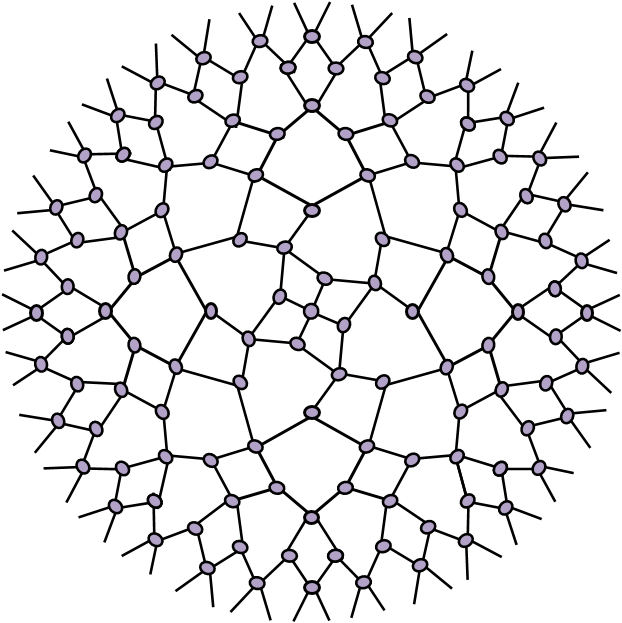
\includegraphics[width=0.5\textwidth]{mera.png}
      \end{figure}
    \end{column}
  \end{columns}

  \begin{itemize} \setlength{\itemsep}{1em}
  \item Machine learning
    \vspace{.51em}
    \begin{itemize}
    \item Data classification, generative modeling
    \end{itemize}

  \item Physics
    \vspace{.5em}
    \begin{itemize}
    \item Correlated quantum matter, quantum gravity
    \end{itemize}
  \end{itemize}

  \uncover<2->{
    \begin{align*}
      v = &\sum_j v_{\color<5->{blue} j} \uv e_j
      &
      M = &\sum_{j,k} M_{\color<5->{blue} jk} \uv e_j \otimes \uv e_k
      &
      \uncover<3->{
        &T_{\color<5->{blue} jk\ell m}
      } \\
      \uncover<4->{
        &\diagram{
          \wire{0}{0}{1};
          \uncover<5->{
            \wire[blue,thick]{0}{0}{1};
          }
          \circ{0}{0}{v};
        }
        &
        &\diagram{
          \wire{0}{-1}{1};
          \uncover<5->{
            \wire[blue,thick]{0}{-1}{1};
          }
          \circ{0}{0}{M};
        }
        &
        &\diagram{
          \dwire{-.75}{+.75}{-.75}{.75};
          \dwire{+.75}{-.75}{-.75}{.75};
          \uncover<5->{
            \dwire[blue,thick]{-.75}{+.75}{-.75}{.75};
            \dwire[blue,thick]{+.75}{-.75}{-.75}{.75};
          }
          \circ{0}{0}{T};
        }
      }
    \end{align*}
  }
\end{frame}

\begin{frame}
  \frametitle{Evaluating a tensor network}

  \vspace{1em}
  Edge contraction
  \begin{align*}
    \diagram{
      \wire{0}{0}{1};
      \wire{0}{2}{3};
      \uncover<2->{
        \wire[red,thick]{0}{1}{2};
      }
      \dwire{0}{+.75}{3}{3.75};
      \dwire{0}{-.75}{3}{3.75};
      \uncover<5->{
        \dwire[blue,thick]{0}{+.75}{3}{3.75};
        \dwire[blue,thick]{0}{-.75}{3}{3.75};
      }
      \circ{0}{0}{v};
      \circ{0}{3}{R};
    }
    \uncover<4->{
      ~ = ~
      \diagram{
        \dwire{0}{+.75}{0}{.75};
        \dwire{0}{-.75}{0}{.75};
        \uncover<5->{
          \dwire[blue,thick]{0}{+.75}{0}{.75};
          \dwire[blue,thick]{0}{-.75}{0}{.75};
        }
        \circ{0}{0}{S};
      }
    }
    \uncover<3->{
      &&
      \to
      &&
      \sum_{\color{red} j} v_{\color{red} j}
      R_{{\color{red} j}{\color<5->{blue} k\ell}}
    }
    \uncover<4->{
      = S_{\color<5->{blue} k\ell}
    }
  \end{align*}

  \vspace{-1em}
  \begin{columns}
    \begin{column}{0.5\textwidth}
      \uncover<6->{
        \begin{align*}
          \uncover<7->{{\color<9-14>{gray} X = ~}}
          \diagram{
            \newcommand{\lblA}{}
            \newcommand{\lblB}{}
            \newcommand{\lblC}{}
            \newcommand{\lblD}{}
            \newcommand{\lblE}{}
            \newcommand{\lblF}{}
            \newcommand{\clrA}{tenblue}
            \newcommand{\clrB}{tenblue}
            \newcommand{\clrC}{tenblue}
            \newcommand{\clrD}{tenblue}
            \newcommand{\clrE}{tenblue}
            \newcommand{\clrF}{tenblue}
            \newcommand{\pthA}{}
            \newcommand{\pthB}{}
            \newcommand{\pthC}{}
            \newcommand{\pthD}{}
            \newcommand{\pthE}{}
            \newcommand{\pthF}{}
            \only<8->{
              \renewcommand{\lblA}{1}
              \renewcommand{\lblB}{2}
              \renewcommand{\lblC}{3}
              \renewcommand{\lblD}{4}
              \renewcommand{\lblE}{5}
              \renewcommand{\lblF}{6}
            }
            \only<9>{
              \renewcommand{\clrB}{tengray}
              \renewcommand{\pthB}{dotted}
            }
            \only<9-10>{
              \renewcommand{\clrC}{tengray}
              \renewcommand{\pthC}{dotted}
            }
            \only<9-11>{
              \renewcommand{\clrD}{tengray}
              \renewcommand{\pthD}{dotted}
            }
            \only<9-12>{
              \renewcommand{\clrE}{tengray}
              \renewcommand{\pthE}{dotted}
            }
            \only<9-13>{
              \renewcommand{\clrF}{tengray}
              \renewcommand{\pthF}{dotted}
            }
            %
            \coordinate (A) at (0,0);
            \coordinate (B) at (2,1);
            \coordinate (C) at (0,2);
            \coordinate (D) at (2,3);
            \coordinate (E) at (4,1);
            \coordinate (F) at (4,3);
            %
            \coordinate (AB) at ($ (A) !.5! (B) $);
            \coordinate (BC) at ($ (B) !.5! (C) $);
            \coordinate (BD) at ($ (B) !.5! (D) $);
            \coordinate (BE) at ($ (B) !.5! (E) $);
            \coordinate (CD) at ($ (C) !.5! (D) $);
            \coordinate (DE) at ($ (D) !.5! (E) $);
            \coordinate (DF) at ($ (D) !.5! (F) $);
            \coordinate (EF) at ($ (E) !.5! (F) $);
            %
            \coordinate (AAB) at ($ (A) !.7! (AB) $);
            \coordinate (ABB) at ($ (AB) !.3! (B) $);
            \coordinate (BBC) at ($ (B) !.7! (BC) $);
            \coordinate (BCC) at ($ (BC) !.3! (C) $);
            \coordinate (BBD) at ($ (B) !.7! (BD) $);
            \coordinate (BDD) at ($ (BD) !.3! (D) $);
            \coordinate (BBE) at ($ (B) !.7! (BE) $);
            \coordinate (BEE) at ($ (BE) !.3! (E) $);
            \coordinate (CCD) at ($ (C) !.7! (CD) $);
            \coordinate (CDD) at ($ (CD) !.3! (D) $);
            \coordinate (DDE) at ($ (D) !.7! (DE) $);
            \coordinate (DEE) at ($ (DE) !.3! (E) $);
            \coordinate (DDF) at ($ (D) !.7! (DF) $);
            \coordinate (DFF) at ($ (DF) !.3! (F) $);
            \coordinate (EEF) at ($ (E) !.7! (EF) $);
            \coordinate (EFF) at ($ (EF) !.3! (F) $);
            %
            \draw[\pthB] (A) -- (B);
            \draw[\pthC] (B) -- (C);
            \draw[\pthD] (B) -- (D);
            \draw[\pthE] (B) -- (E);
            \draw[\pthD] (C) -- (D);
            \draw[\pthE] (D) -- (E);
            \draw[\pthF] (D) -- (F);
            \draw[\pthF] (E) -- (F);
            %
            \only<9>{
              \draw[blue,thick] (A) -- (AB);
            }
            \only<10>{
              \draw[blue,thick] (B) -- (BC);
            }
            \only<10-11>{
              \draw[blue,thick] (B) -- (BD);
            }
            \only<10-12>{
              \draw[blue,thick] (B) -- (BE);
            }
            \only<11>{
              \draw[blue,thick] (C) -- (CD);
            }
            \only<12>{
              \draw[blue,thick] (D) -- (DE);
            }
            \only<12-13>{
              \draw[blue,thick] (D) -- (DF);
            }
            \only<13>{
              \draw[blue,thick] (E) -- (EF);
            }
            %
            \only<10>{
              \draw[red,thick] (AAB) -- (ABB);
            }
            \only<11>{
              \draw[red,thick] (BBC) -- (BCC);
            }
            \only<12>{
              \draw[red,thick] (BBD) -- (BDD);
              \draw[red,thick] (CCD) -- (CDD);
            }
            \only<13>{
              \draw[red,thick] (BBE) -- (BEE);
              \draw[red,thick] (DDE) -- (DEE);
            }
            \only<14>{
              \draw[red,thick] (DDF) -- (DFF);
              \draw[red,thick] (EEF) -- (EFF);
            }
            %
            \draw[\clrA] (A) circle (0.5) node {\lblA};
            \draw[\clrB] (B) circle (0.5) node {\lblB};
            \draw[\clrC] (C) circle (0.5) node {\lblC};
            \draw[\clrD] (D) circle (0.5) node {\lblD};
            \draw[\clrE] (E) circle (0.5) node {\lblE};
            \draw[\clrF] (F) circle (0.5) node {\lblF};
          }
        \end{align*}
      }
    \end{column}
    \begin{column}{0.5\textwidth}
      \uncover<16->{
        \begin{align*}
          \diagram{
            \dwire{0}{+2}{0}{4};
            \dwire{0}{-2}{0}{4};
            \dwire{+1}{0}{2}{4};
            \dwire{-1}{0}{2}{4};
            %
            \dwire[dotted]{+2}{+3.5}{4}{7};
            \dwire[dotted]{+2}{+0.5}{4}{7};
            \dwire[dotted]{-2}{-0.5}{4}{7};
            \dwire[dotted]{-2}{-3.5}{4}{7};
            \dwire[dotted]{0}{+1.5}{4}{7};
            \dwire[dotted]{0}{-1.5}{4}{7};
            \dwire[dotted]{+3}{+2.5}{6}{7};
            \dwire[dotted]{-3}{-2.5}{6}{7};
            %
            \dwire[blue,thick]{+2}{+2.5}{4}{5};
            \dwire[blue,thick]{+2}{+1.5}{4}{5};
            \dwire[blue,thick]{-2}{-1.5}{4}{5};
            \dwire[blue,thick]{-2}{-2.5}{4}{5};
            \dwire[blue,thick]{0}{+.5}{4}{5};
            \dwire[blue,thick]{0}{-.5}{4}{5};
            %
            \circ{0}{0}{};
            \circ{+1}{2}{};
            \circ{-1}{2}{};
            \circ{-2}{4}{};
            \circ{+0}{4}{};
            \circ{+2}{4}{};
            \circ[tengray]{+3}{6}{};
            \circ[tengray]{+1}{6}{};
            \circ[tengray]{-1}{6}{};
            \circ[tengray]{-3}{6}{};
          }
        \end{align*}
      }
    \end{column}
  \end{columns}
  \uncover<17>{
    \begin{center}
      Exponential memory requirements!
    \end{center}
  }
\end{frame}

\begin{frame}
  \frametitle{Quantum computers}
  \begin{itemize} \setlength{\itemsep}{1em}
  \item $N$ qubits $\to$ $2^N$-dimensional state space
    \begin{align*}
      \ket\psi = \sum_{j,k,\ell,\cdots}
      \psi_{jk\ell\cdots} \ket{jk\ell\cdots}
      \uncover<2->{
        = ~
        \diagram{
          \wire{1.5}{0}{2};
          \wire{+.5}{0}{2};
          \wire{-1.5}{0}{2};
          \draw (1.9,-.3) node {$\vdots$};
          \rect{-2}{2}{0}{1.5}{\psi};
        }
      }
    \end{align*}

  \item<3-> Quantum circuit: {\it unitary} tensor network
    \begin{align*}
      \diagram{
        \wire{0}{-.5}{3.5};
        \wire{1.5}{-.5}{3.5};
        \wire{-1.5}{-.5}{3.5};
        \rect[tengray]{1}{2}{0}{1}{H};
        \cnot{1.75}{1.5}{0};
        \cnot{2.75}{0}{-1.5};
        \draw (-1,0) node {$\ket{0}$};
        \draw (-1,1.5) node {$\ket{0}$};
        \draw (-1,-1.5) node {$\ket{0}$};
      }
      ~ = ~
      \diagram{
        \wire{0}{-.5}{4.5};
        \wire{1.5}{-.5}{4.5};
        \wire{-1.5}{-.5}{4.5};
        \rect{-.5}{.5}{-1.5}{-.5}{0};
        \rect{1}{2}{-1.5}{-.5}{0};
        \rect{-2}{-1}{-1.5}{-.5}{0};
        \rect[tenorange]{1}{2}{0}{1}{};
        \rect[tenorange]{-.5}{2}{1.5}{2.5}{};
        \rect[tenorange]{-2}{.5}{3}{4}{};
      }
      ~ = ~
      \diagram{
        \wire{+1}{0}{2.5};
        \wire{-1}{0}{2.5};
        \wire{0}{0}{2.5};
        \rect{-2}{2}{0}{2}{\psi_{\t{GHZ}}};
      }
    \end{align*}

  \item<4-> Tricks for computing non-unitary tensor networks ~\hfill
    \uncover<5->{(!!!)}
  \end{itemize}
\end{frame}

\begin{frame}
  \frametitle{Partition function}
  \begin{align*}
    Z = \sum_{\substack{\t{all physical}\\\t{state}}} e^{-E/T}
  \end{align*}

  \begin{itemize} \setlength{\itemsep}{1em}
  \item Energy $E$: function of state

  \item Summarizes all equilibrium physics at temperature $T$

    \vspace{.5em}
    \begin{itemize}
    \item Mean energy, magnetization, heat capacity, etc.
    \end{itemize}

  \item<2-> Tensor network representation
    \begin{align*}
      Z =
      \diagram{
        \wire{0}{-1}{2.5};
        \wire{1.5}{-1}{2.5};
        \vwire{0}{-1}{2.5};
        \vwire{1.5}{-1}{2.5};
        %
        \circ{0}{0}{T};
        \circ{0}{1.5}{T};
        \circ{1.5}{0}{T};
        \circ{1.5}{1.5}{T};
        %
        \draw (-1.75,0) node {$\cdots$};
        \draw (-1.75,1.5) node {$\cdots$};
        \draw (3.25,0) node {$\cdots$};
        \draw (3.25,1.5) node {$\cdots$};
        %
        \draw (0,-1.5) node {$\vdots$};
        \draw (1.5,-1.5) node {$\vdots$};
        \draw (0,3.25) node {$\vdots$};
        \draw (1.5,3.25) node {$\vdots$};
      }
    \end{align*}
  \end{itemize}
\end{frame}

\begin{frame}
  \frametitle{The $q$-state clock (Potts) model}
  \vspace{-1em}
  \uncover<3->{
    \tikz[remember picture,overlay]{
      \node[anchor=south east] at (current page.south east)
      {\includegraphics[width=0.4\textwidth]{clock_network.pdf}};
    }
  }
  \begin{columns}
    \begin{column}{0.75\textwidth}
      \begin{itemize} \setlength{\itemsep}{1em}
      \item Spins $\v s=\p{\cos\theta,\sin\theta}$
      \item<2-> $q$ discrete angles $\theta\in\Z\times2\pi/q$
        \uncover<3->{
          \vspace{1.5em}
          \begin{align*}
            E &= -\sum_{\substack{\t{neighbors}\\\bk{j,k}}}
            {\color<4>{red}
              \uubrace<4->{\v s_j\c\v s_k}
              {\substack{\t{interaction}\\\t{(spin aligment)}}}
            }
            - \sum_{\t{sites}~\ell}
            {\color<5>{red}
              \uubrace<5->{\v h\c\v s_\ell}
              {\substack{\t{``magnetic'' field}\\\t{(global bias)}}}
            }
            \\[.5em]
            \uncover<6->{
              &= -\sum_{\bk{j,k}} \cos\p{\theta_j-\theta_k}
              - h \sum_\ell \cos\theta_\ell
            }
          \end{align*}
        }
        \vspace{-1em}
      \item<7-> Ising model: $q=2$
      \item<7-> Classical XY model: $q\to\infty$
      \end{itemize}
    \end{column}
    \begin{column}{0.25\textwidth}
      \begin{figure}
        \centering
        \uncover<2->{
          \includegraphics[width=\textwidth]{clock.pdf}
          \caption{12-state clock}
        }
      \end{figure}
      \vspace{1.3\textwidth}~
    \end{column}
  \end{columns}
\end{frame}

\begin{frame}
  \frametitle{The punchline}

  \vspace{1em}
  Output of quantum computation: prob.~$p$ of finding all qubits in
  $\ket{0}$

  \vspace{-1em}
  \begin{align*}
    Z \propto \sqrt{p}
  \end{align*}

  \vspace{-.5em}
  \uncover<2->{
    \begin{figure}
      \centering
      \includegraphics<1-2>[width=0.7\textwidth]{probs_example.pdf}

      \includegraphics<3->[width=0.7\textwidth]{probs_example_refs.pdf}
    \end{figure}
  }

  \vspace{-1em}
  \uncover<4->{
    \begin{center}
      Natural sensitivity to phase transitions!
    \end{center}
  }
\end{frame}

\begin{frame}[plain]
  ~ \vfill
  \begin{center}
    \large \bf Thank you
  \end{center}
  \vfill ~
\end{frame}
\addtocounter{framenumber}{-1}

\end{document}
